%-----------------------------------------------------------------------------------------------
\makeatletter
\immediate\write18{datelog > \jobname.info} % site script for $(date '+%Y-%m-%d %Hh%Mm%Ss')
\makeatother
%-----------------------------------------------------------------------------------------------
%-----------------------------------------------------------------------------------------------
\usetheme{Copenhagen}
\usepackage{beamercolorthemeCNThermSci2}
\usefonttheme{serif}
%-----------------------------------------------------------------------------------------------

%-----------------------------------------------------------------------------------------------
%-----------------------------------------------------------------------------------------------
\usetheme{Copenhagen}
\usepackage{beamercolorthemeUTF2}
\usefonttheme{serif}
%-----------------------------------------------------------------------------------------------
\usepackage[utf8]{inputenc}
\usepackage[greek,french,english,brazil]{babel} % last becomes the active one
\usepackage{pslatex}
\usepackage{amssymb,amsmath}
\usepackage{soul}
\usepackage[squaren,Gray,cdot]{SIunits}
\usepackage[nice]{nicefrac}
\usepackage{tikz}
\usepackage{amscd}
\usepackage{stmaryrd}
\usepackage{scalerel}
\usepackage{xspace}
%-----------------------------------------------------------------------------------------------


%-----------------------------------------------------------------------------------------------
%-----------------------------------------------------------------------------------------------
% Mathematical
%-----------------------------------------------------------------------------------------------
\newcommand{\vet}[1]{\underline{{#1}}}
\newcommand{\mat}[1]{\underline{\underline{{#1}}}}
\newcommand{\cub}[1]{\underline{\underline{\underline{{#1}}}}}
\newcommand{\eqdef}{{\ensuremath\stackrel{\text{\tiny def}}{=}}}
%-----------------------------------------------------------------------------------------------
% Linguistic
%-----------------------------------------------------------------------------------------------
\newcommand{\GRtxt}[1]{\begin{otherlanguage}{greek}{{#1}}\end{otherlanguage}}
\newcommand{\FRtxt}[1]{\begin{otherlanguage}{french}{{#1}}\end{otherlanguage}}
%-----------------------------------------------------------------------------------------------
% Presentation
%-----------------------------------------------------------------------------------------------
\newcommand{\BkgImgH}[1]{% Places an image centered on the slide background filling the height
    \usebackgroundtemplate{\parbox{\paperwidth}{%
        \vspace*{1sp}\centering\includegraphics[height=\paperheight]{{#1}}
}}}
\newcommand{\BkgImgW}[1]{% Places an image centered on the slide background filling the width
    \usebackgroundtemplate{\parbox{\paperwidth}{%
        \vspace*{1sp}\centering\includegraphics[width=\paperwidth]{{#1}}
}}}
\newcommand{\ArtEndH}[3]{% Transitions to plain image (last) slide: #1:prefix #2,#3:extensions
    \BkgImgH{root/../art/#1.#2}
    \frame<handout:0>[plain]{%
        \transdissolve\vspace*{72mm}\color{white}\scriptsize\bf\input{root/../art/#1.#3}}
    \usebackgroundtemplate{\mbox{~}}
}
\newcommand{\ArtEndW}[3]{% Transitions to plain image (last) slide: #1:prefix #2,#3:extensions
    \BkgImgW{root/../art/#1.#2}
    \frame<handout:0>[plain]{%
        \transdissolve\vspace*{72mm}\color{white}\scriptsize\bf\input{root/../art/#1.#3}}
    \usebackgroundtemplate{\mbox{~}}
}
\newcommand{\ImgColW}[3]{% Inserts a full-width image in a column
    \includegraphics[width=\columnwidth]{root/../art/#1.#2}\\[-0.5\baselineskip]
    \parbox{\columnwidth}{\tiny\hfill\scalebox{0.85}{\input{root/../art/#1.#3}}}
}
\newcommand{\txtpic}[1]{%
    \fcolorbox{lightgray}{white!90!black}{{#1}} 
}
%-----------------------------------------------------------------------------------------------


%-----------------------------------------------------------------------------------------------
\newcommand{\VPMS}{{\ensuremath V_{\mathrm{PMS}}}}
\newcommand{\VPMI}{{\ensuremath V_{\mathrm{PMI}}}}
%-----------------------------------------------------------------------------------------------
\title{An Inertial Air-standard Finite-time Heat\\ Addition Otto Engine Model}
\subtitle{ENC-2020-0067}
\author{F.~M.~Moreira and Prof.~C.~Naaktgeboren, PhD}
\date{{\scriptsize\tt%
    
\includegraphics[height=6.0mm]{root/00-res/cc/by-nc-nd-88x31.pdf}\\[\smallskipamount]
    https://github.com/CNThermSci/ApplThermSci\\
    Compiled on \input{\jobname.info}
}}
%-----------------------------------------------------------------------------------------------
\begin{document}
%-----------------------------------------------------------------------------------------------
\logo{%
    \parbox{158mm}{% There's a 1mm gap on each side of the 160mm x 90mm slide logo line
        \mode<beamer>{
            
\includegraphics[height=6.0mm]{root/00-res/UTFPR/UTFPR-logo-D.pdf}\hfill%
            
\includegraphics[height=9.0mm]{root/00-res/logo/CNThermSci-logo-A.pdf}%
        }
        \mode<handout>{
            
\includegraphics[height=6.0mm]{root/00-res/UTFPR/UTFPR-logo-W.pdf}\hfill%
            
\includegraphics[height=9.0mm]{root/00-res/logo/CNThermSci-logo-W.pdf}%
        }
    }
} % The (delineated, alpha), or washed-out logos
%-----------------------------------------------------------------------------------------------
\frame{\titlepage}
\frame{\tableofcontents}
%-----------------------------------------------------------------------------------------------

%-----------------------------------------------------------------------------------------------
\section{iFTHA Modeling}
%-----------------------------------------------------------------------------------------------

%-----------------------------------------------------------------------------------------------
\subsection{Introduction}
%-----------------------------------------------------------------------------------------------

    % !j 96 -i8
    %-------------------------------------------------------------------------------------------
    \begin{frame}{iFTHA}\vspace*{-2em}
        \uncover<1->{The work proposes a}\vspace*\medskipamount
        \begin{itemize}
            \item<1->  fairly simple \alert{coupled dynamic-thermodynamic} engine model, i.e.,
            \item<1->  an \alert{inertial}, \alert{air-standard}, Otto model with:
            \item<1->  \alert{finite-time} heat release,
            \item<1->  basic \alert{engine parameters}, and
            \item<1->  \alert{piston}, \alert{rod}, \alert{crank}, and \alert{flywheel}
                inertias.
        \end{itemize}
    \end{frame}
    %-------------------------------------------------------------------------------------------

    % !j 96 -i8
    %-------------------------------------------------------------------------------------------
    \begin{frame}{Motivation}\vspace*{-2em}
        \uncover<1->{
            \alert{Dynamic extension} of a somewhat recently \alert{published}$^\dagger$
            \alert{FTHA} model:
        }%
        \vspace*\medskipamount
        \begin{itemize}
            \item<1->  \alert{air-standard reversible}, \alert{finite-time} heat release, Otto
                engine (spark-ignited) model:
            \item<1->  \alert{minimal-complexity}, \alert{pure-substance} model
            \item<1->  including \alert{simultaneous heat+work} interactions.
            \item<2->  \alert{Differs} from other literature works
            \item<2->  by the \alert{early removal} of the \alert{isochoric} heating of the
                ideal Otto model;
            \item<2->  ...thus able to reproduce cycles with \alert{$P$-$v$} diagrams as
                following:
        \end{itemize}\vspace*\bigskipamount
        {\footnotesize$^\dagger$~\color{Lgre}
        Naaktgeboren, C. \textbf{Int.~J.~Mech.~Eng.~Educ.}, 45(2), 2017.}
    \end{frame}
    %-------------------------------------------------------------------------------------------

    % !j 96 -i8
    %-------------------------------------------------------------------------------------------
    \begin{frame}\vspace*{-2em}
        \begin{center}
            \noindent\hspace*{-4.5mm}%
            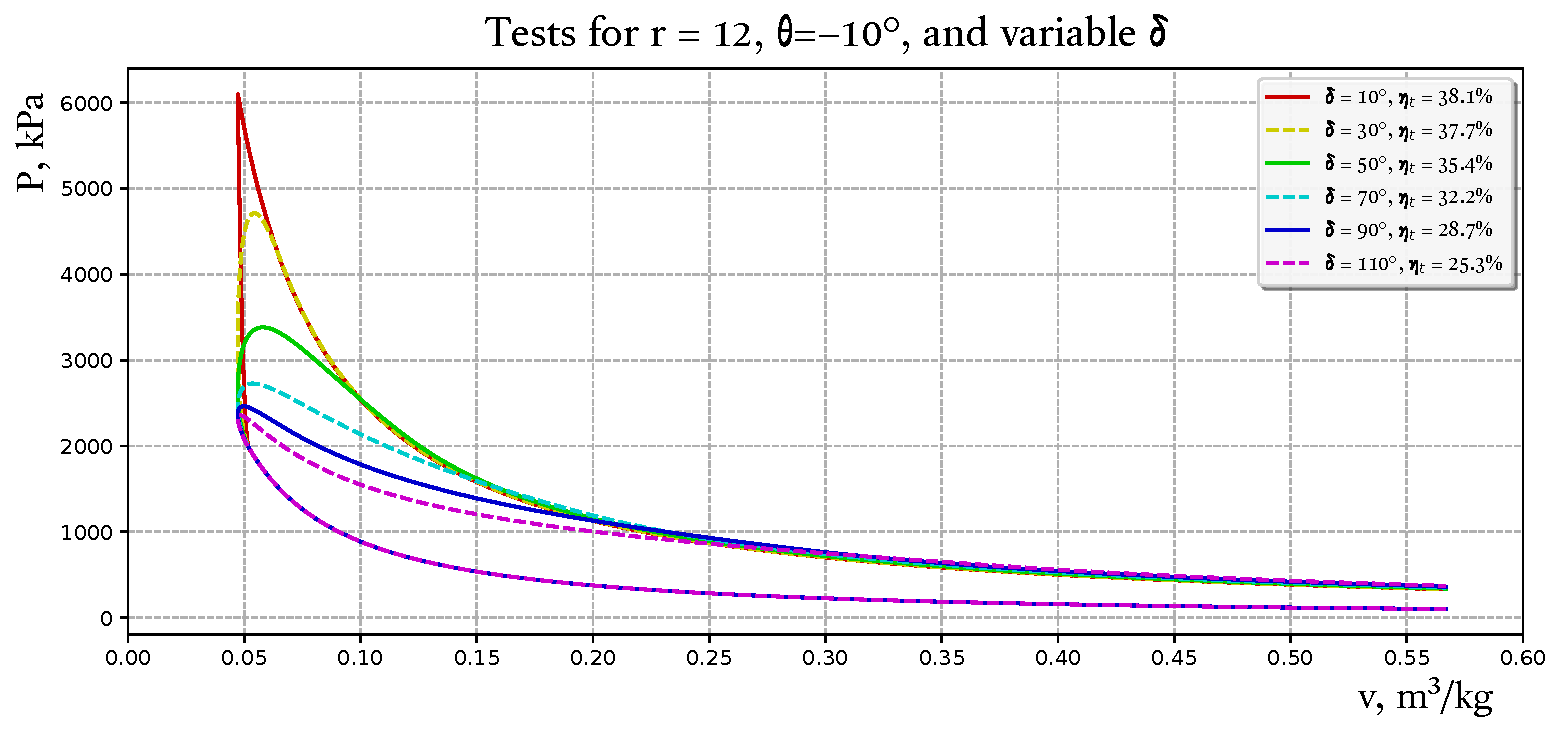
\includegraphics[height=70.0mm]{01-FTHA/fig/test_r=12,0_speed-P.pdf}
        \end{center}
    \end{frame}
    %-------------------------------------------------------------------------------------------

    % !j 96 -i8
    %-------------------------------------------------------------------------------------------
    \begin{frame}{Strategy}\vspace*{-2em}
        \uncover<1->{Merge between the \alert{FTHA} and a \alert{suitable dynamic}
        model:}\\[\medskipamount]
        \uncover<1->{Const-velocity, \alert{one-way coupling} models:}%
        \vspace*\medskipamount
        \begin{itemize}
            \item<1->  very simple \alert{lumped}, translation-\alert{only} components;
            \item<1->  mathematically more complex, external tools, and elastic ones.
        \end{itemize}
        \vspace*\medskipamount
        \uncover<1->{Variable-velocity, \alert{two-way coupling}, rigid body inertial model of:}%
        \vspace*\medskipamount
        \begin{itemize}
            \item<1->  rigid body inertial model due to \alert{Montazersadgh}$^\ddagger$.
        \end{itemize}
        \vspace*\medskipamount
        {\footnotesize$^\ddagger$~\color{Lgre}
        Montazersadgh, F.~H. MSc Thesis, \textbf{U.~Toledo}, 2007.}
    \end{frame}
    %-------------------------------------------------------------------------------------------

%-----------------------------------------------------------------------------------------------
\subsection{Thermodynamic Modeling}
%-----------------------------------------------------------------------------------------------

    % !j 96 -i8
    %-------------------------------------------------------------------------------------------
    \begin{frame}{Thermodynamic Modeling}\vspace*{-2em}
        \begin{columns}
        \column{0.75\textwidth}
            \uncover<1->{Engine model input \alert{parameters}:}
            \only<1>{
                \begin{itemize}
                    \item Crank radius \alert{$R$};
                    \item Crank position \alert{$\alpha$} and velocity \alert{$\omega$};$\qquad$(CCW)
                    \item Rod length \alert{$L$};
                    \item Piston diameter \alert{$D$} and stroke \alert{$S=2R$};
                    \item Top Dead Center (TDC) volume, \alert{$V_{min}$};
                    \item Bottom Dead Center (BDC) volume, \alert{$V_{max}$};
                    \item Engine compression ratio, \alert{$r=\nicefrac{V_{max}}{V_{min}}$};
                \end{itemize}
            }
            \only<2>{
                \begin{itemize}
                    \item Crank position \alert{$\alpha$} and velocity \alert{$\omega$};$\qquad$(CCW)
                    \item Rod length \alert{$L$};
                    \item Piston diameter \alert{$D$} and stroke \alert{$S=2R$};
                    \item Top Dead Center (TDC) volume, \alert{$V_{min}$};
                    \item Bottom Dead Center (BDC) volume, \alert{$V_{max}$};
                    \item Engine compression ratio, \alert{$r=\nicefrac{V_{max}}{V_{min}}$};
                    \item Engine displaced volume, \alert{$V_{d}$};
                \end{itemize}
            }
            \only<3>{
                \begin{itemize}
                    \item Rod length \alert{$L$};
                    \item Piston diameter \alert{$D$} and stroke \alert{$S=2R$};
                    \item Top Dead Center (TDC) volume, \alert{$V_{min}$};
                    \item Bottom Dead Center (BDC) volume, \alert{$V_{max}$};
                    \item Engine compression ratio, \alert{$r=\nicefrac{V_{max}}{V_{min}}$};
                    \item Engine displaced volume, \alert{$V_{d}$};
                    \item Cylinder count \alert{$z$}, and unit displaced volume,
                        \alert{$V_{du}=V_d/z$};
                \end{itemize}
            }
        \column{0.25\textwidth}

        \vspace*{-4mm}% Prev+After lines needs to be a blank one as to ensure vertical mode
        \hspace*{-6mm}\includegraphics[width=\textwidth]{src/FIG_mechanism_rev05.pdf}

        \end{columns}
    \end{frame}
    %-------------------------------------------------------------------------------------------

    % !j 96 -i8
    %-------------------------------------------------------------------------------------------
    \begin{frame}{Thermodynamic Modeling}\vspace*{-2em}
        \begin{columns}
        \column{0.75\textwidth}
            \uncover<1->{
                \begin{align*}
                    \alert{x(\alpha)} &
                    \alert{= L\left[1-\sqrt{1-\left(\frac{R\sin\alpha}{L}\right)^2}\right]
                        + R(1-\cos\alpha)},
                    \\[\medskipamount]
                    \alert{V(\alpha)} &
                    \alert{= V_{min} + \frac{\pi D^2}{4}x(\alpha)},
                    \\[\medskipamount]
                    \alert{v(\alpha)} &
                    \alert{= \frac{V(\alpha)}{m}},\qquad\mbox{with}\qquad
                    \alert{m = \frac{P_0V_0}{RT_0}},
                    \\[\medskipamount]
                    \alert{t_{i+1}} &
                    \alert{= t_i + \Delta{t}},\qquad\mbox{and}\qquad
                    \alert{\alpha_{i+1} = \alpha_i + \omega\Delta{t}}.
                \end{align*}
            }
        \column{0.25\textwidth}

        \vspace*{-4mm}% Prev+After lines needs to be a blank one as to ensure vertical mode
        \hspace*{-6mm}\includegraphics[width=\textwidth]{src/FIG_mechanism_rev05.pdf}

        \end{columns}
    \end{frame}
    %-------------------------------------------------------------------------------------------

    % !j 96 -i8
    %-------------------------------------------------------------------------------------------
    \begin{frame}{Thermodynamic Modeling}\vspace*{-2em}
        \begin{columns}
        \column{0.75\textwidth}
            \uncover<1->{
                \begin{align*}
                    \alert{q_i + w_i} &
                    \alert{= \Delta u_i = u_{i+1} - u_i},
                    \\[\medskipamount]
                    \alert{y(t^{\star})} &
                    \alert{= \begin{cases}
                        0,              & \mbox{for $t^{\star} < t^{\star}_{\theta}$,} \\
                        g(t^{\star}),   & \mbox{for
                            $t^{\star}_{\theta} \leqslant t^{\star} < t^{\star}_{\theta} + \Delta{t_c}$,
                        } \\
                        1,              & \mbox{for $t^{\star}_{\theta} + \Delta{t_c} \leqslant t^{\star}$.}
                    \end{cases}}
                    \\[\medskipamount]
                    \alert{q_i} &
                    \alert{= q_{ent}\Delta{y_i}},\qquad\mbox{with}
                    \\[\medskipamount]
                    \alert{\Delta{y_i}} &
                    \alert{=y(t^{\star}_{i+1})-y(t^{\star})},
                    \\[\medskipamount]
                    \alert{\alpha(t^{\star}_{\theta})} &
                    \alert{= \theta},\qquad\mbox{and}
                    \\[\medskipamount]
                    \alert{t^{\star}} &
                    \alert{\leftarrow 0}\qquad\mbox{whenever}\qquad
                    \alert{(\alpha \mod 2\pi) = 0}.
                \end{align*}
            }
        \column{0.25\textwidth}

        \vspace*{-4mm}% Prev+After lines needs to be a blank one as to ensure vertical mode
        \hspace*{-6mm}\includegraphics[width=\textwidth]{src/FIG_mechanism_rev05.pdf}

        \end{columns}
    \end{frame}
    %-------------------------------------------------------------------------------------------

    % !j 96 -i8
    %-------------------------------------------------------------------------------------------
    \begin{frame}{Thermodynamic Modeling}\vspace*{-2em}
        \begin{columns}
        \column{0.75\textwidth}
            \uncover<1->{
                \begin{align*}
                    \alert{u_{i+1}^j} &
                    \alert{= u_i + q_i + w_i^j},\quad\mbox{with}
                    \\[\smallskipamount]
                    w_i^j & =
                        \begin{cases}
                            \frac{P_iv_i}{1-n_i^j}\cdot\biggl[
                                1 - \Bigl(
                                    \frac{v_i}{v_{i+1}}
                                \Bigr)^{\scriptstyle{n_i^j-1}}
                            \biggr],\quad &
                            \mathrm{for}\quad n_i^j \neq 1 \\[\medskipamount]
                            P_i\cdot v_i\cdot\ln\Bigl(
                                \frac{v_i}{v_{i+1}}
                            \Bigr),\quad &
                            \mathrm{for}\quad n_i^j = 1
                        \end{cases}
                    \\[\smallskipamount]
                    T_{i+1}^j & = f(u_{i+1}^j, c_v(T), v_{i+1}),
                    \\[\smallskipamount]
                    P_{i+1}^j & = f(T_{i+1}^j, v_{i+1}),\quad\mbox{finally correcting for $n_i^j$ with}
                    \\[\smallskipamount]
                    n_i^{j+1} & = \Bigl(
                        \log\textstyle\frac{P_{i+1}^j}{P_i}
                    \Bigr)\Bigl/\Bigr.\Bigl(
                        \log\textstyle\frac{v_i}{v_{i+1}}
                    \Bigr).
                \end{align*}
            }
        \column{0.25\textwidth}

        \vspace*{-4mm}% Prev+After lines needs to be a blank one as to ensure vertical mode
        \hspace*{-6mm}\includegraphics[width=\textwidth]{src/FIG_mechanism_rev05.pdf}

        \end{columns}
    \end{frame}
    %-------------------------------------------------------------------------------------------

%-----------------------------------------------------------------------------------------------
\subsection{Dynamic Modeling}
%-----------------------------------------------------------------------------------------------

    % !j 96 -i8
    %-------------------------------------------------------------------------------------------
    \begin{frame}{Title}{Subtitle}\vspace*{-2em}
        \uncover<1->{Some text:}
        \begin{itemize}
            \item<2->  A \alert{relevant} item;
            \item<3->  Another \alert{important} point;
        \end{itemize}
    \end{frame}
    %-------------------------------------------------------------------------------------------

%-----------------------------------------------------------------------------------------------
\section{iFTHA Results}
%-----------------------------------------------------------------------------------------------

%-----------------------------------------------------------------------------------------------
\subsection{Validation Results}
%-----------------------------------------------------------------------------------------------

    % !j 96 -i8
    %-------------------------------------------------------------------------------------------
    \begin{frame}{Title}{Subtitle}\vspace*{-2em}
        \uncover<1->{Some text:}
        \begin{itemize}
            \item<2->  A \alert{relevant} item;
            \item<3->  Another \alert{important} point;
        \end{itemize}
    \end{frame}
    %-------------------------------------------------------------------------------------------

%-----------------------------------------------------------------------------------------------
\subsection{Case Study Results}
%-----------------------------------------------------------------------------------------------

    % !j 96 -i8
    %-------------------------------------------------------------------------------------------
    \begin{frame}{Single-Cycle No-load Acceleration}{Subtitle}\vspace*{-2em}
        \uncover<1->{Some text:}
        \begin{itemize}
            \item<2->  A \alert{relevant} item;
            \item<3->  Another \alert{important} point;
        \end{itemize}
    \end{frame}
    %-------------------------------------------------------------------------------------------

    % !j 96 -i8
    %-------------------------------------------------------------------------------------------
    \begin{frame}{Multiple-Cycle No-load Acceleration}{Subtitle}\vspace*{-2em}
        \uncover<1->{Some text:}
        \begin{itemize}
            \item<2->  A \alert{relevant} item;
            \item<3->  Another \alert{important} point;
        \end{itemize}
    \end{frame}
    %-------------------------------------------------------------------------------------------

%-----------------------------------------------------------------------------------------------
\section{Conclusions}
%-----------------------------------------------------------------------------------------------

    % !j 96 -i8
    %-------------------------------------------------------------------------------------------
    \begin{frame}{Title}{Subtitle}\vspace*{-2em}
        \uncover<1->{Some text:}
        \begin{itemize}
            \item<2->  A \alert{relevant} item;
            \item<3->  Another \alert{important} point;
        \end{itemize}
    \end{frame}
    %-------------------------------------------------------------------------------------------

%-----------------------------------------------------------------------------------------------
% End splash screen
%-----------------------------------------------------------------------------------------------

    % Finishes with stunning image, with credit
    \ArtEndW{pexels-alexandre-saraiva-carniato-2309922}{jpg}{txt}

%-----------------------------------------------------------------------------------------------
\end{document}
%-----------------------------------------------------------------------------------------------

